\documentclass{report}
\usepackage[utf8]{inputenc}
\usepackage{graphicx}
\usepackage[siunitx,europeanresistors,american voltages]{circuitikz}
\usepackage{tikz}
\usepackage{pgfplots}
\pgfplotsset{compat=1.7}
\usepackage{adjustbox}
\usepackage{array}
\usepackage{makeidx}
\usepackage{listings}
\usepackage{pgf}
\usepackage{float}
\usepackage[section]{placeins}
\usepackage{wrapfig}
\usepackage[nottoc]{tocbibind} 
\usepackage[english]{babel}


\title{Lab Report 1}
\author{Nedim Hafizovic}
\date{March 2018}

\begin{document}

\maketitle

\tableofcontents

\chapter{Theoretical part}

\section{Circuit calculation}
\vspace{15mm}

\begin{table}[!htb]
\centering
\setlength{\tabcolsep}{30pt}
\setlength{\extrarowheight}{20pt}
\Large
\begin{tabular}{ | c | c | } 

\hline
 \textbf{R1} & 3 \\ 
 \hline
 \textbf{R2} & 7 \\ 
 \hline
 \textbf{V1} & 2,6 \\ 
 \hline
 \textbf{UR1} & 0,78 \\ 
 \hline
 \textbf{UR2} & 1,82 \\ 
 \hline
\end{tabular}
\end{table}

\newpage
\section{Circuit diagram}
\vspace{10mm}
\begin{center}
\begin{circuitikz}[scale=1, every node/.style={transform shape}]
\draw
(0,0) to (6,0)
to [R=7<\ohm>] (6,4) 
to [R=7<\ohm>] (0,4) 
to [battery1={2.6}{V}]  (0,0)
;
\end{circuitikz}
\end{center}

\vspace{2cm}

\section{Circuit plot}
\vspace{10mm}
\begin{center}
\begin{tikzpicture}
\begin{axis}[]

\addplot [black, very thick]{U(R2) = f(R2).};
\end{axis}
\end{tikzpicture}
\end{center}

\newpage
\chapter{Practical part}

\section{Work with GEDA programs}
\newpage
\subsection{Work with gschem}


\begin{figure}[!ht]
\centering
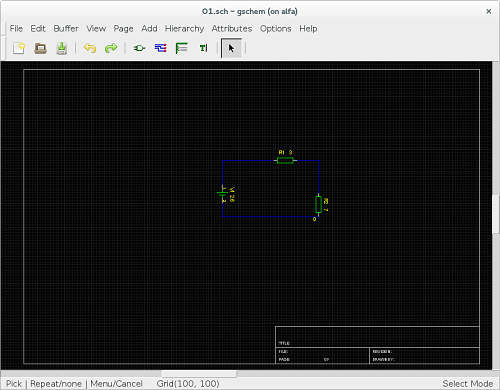
\includegraphics[width=.83\linewidth]{gschem_1}
\caption{Circuit within the gEDA schematics environment. \cite{geda}}
\end{figure}
\vspace*{\floatsep}
\begin{figure}[!hb]
\centering
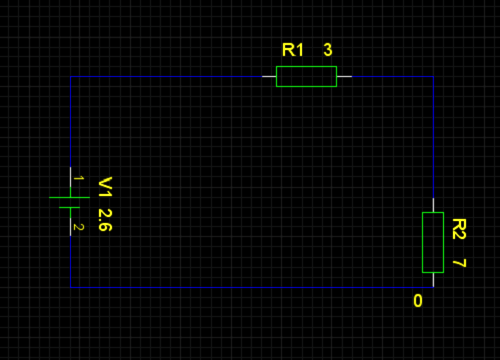
\includegraphics[width=.83\linewidth]{gschem_2}
\caption{Circuit with elements R1, R2 and V1.}
\label{i:gschem}
\end{figure}

\newpage
\subsection{Work with gnetlist}
\lstinputlisting[firstline=1,lastline=10]{01.net}
\newpage

\subsection{Work with ngspice}

\begin{figure}[!ht]
\centering
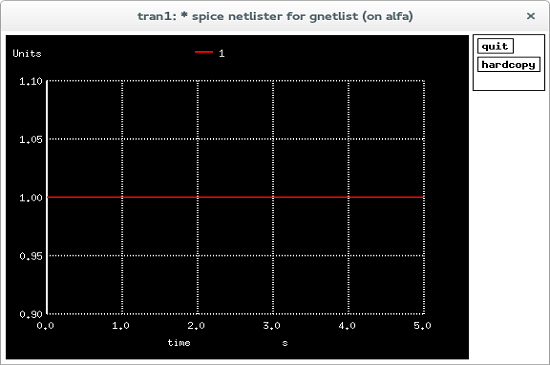
\includegraphics[width=.9\linewidth]{ngspice_1}
\caption{Simulation of voltage on resistor R1.}
\label{i:example2}
\end{figure}
\vspace*{\floatsep}
\begin{figure}[!hb]
\centering
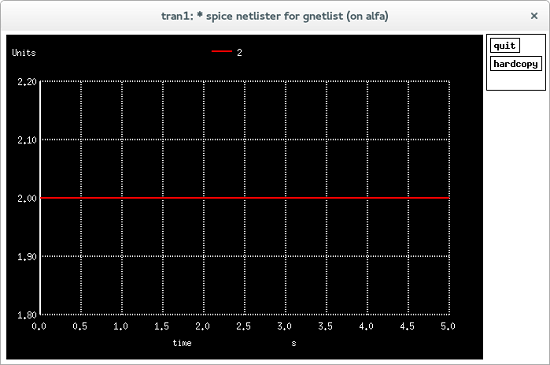
\includegraphics[width=.9\linewidth]{ngspice_2}
\caption{Simulation of voltage on resistor R2.}
\label{i:ngspice}
\end{figure}

\newpage

\section{Work with QUCS programs}
\begin{figure}[!ht]
\centering
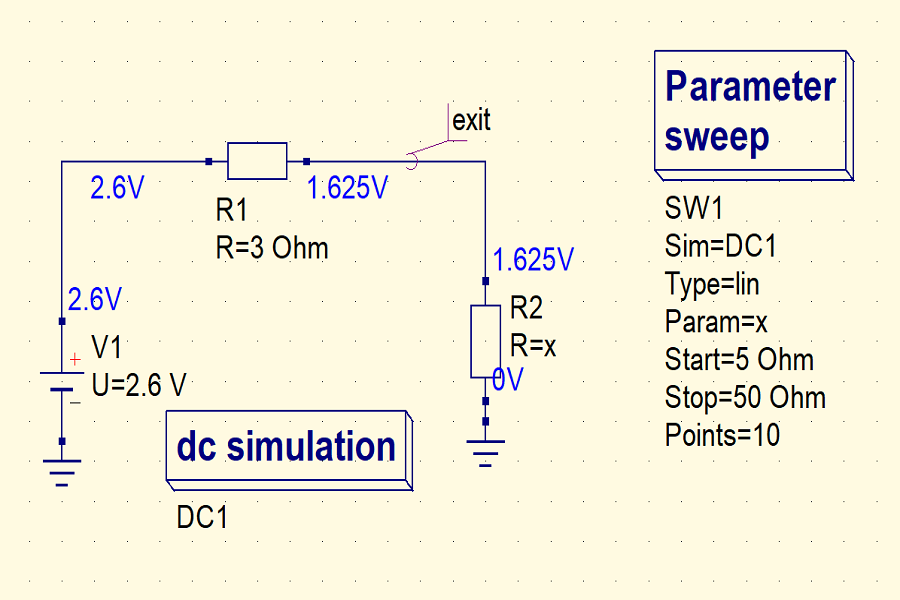
\includegraphics[width=.9\linewidth]{qucs_1}
\caption{Circuit within the QUCS schematics environment. {\cite{qucs}}}
\end{figure}
\vspace*{\floatsep}
\begin{figure}[!hb]
\centering
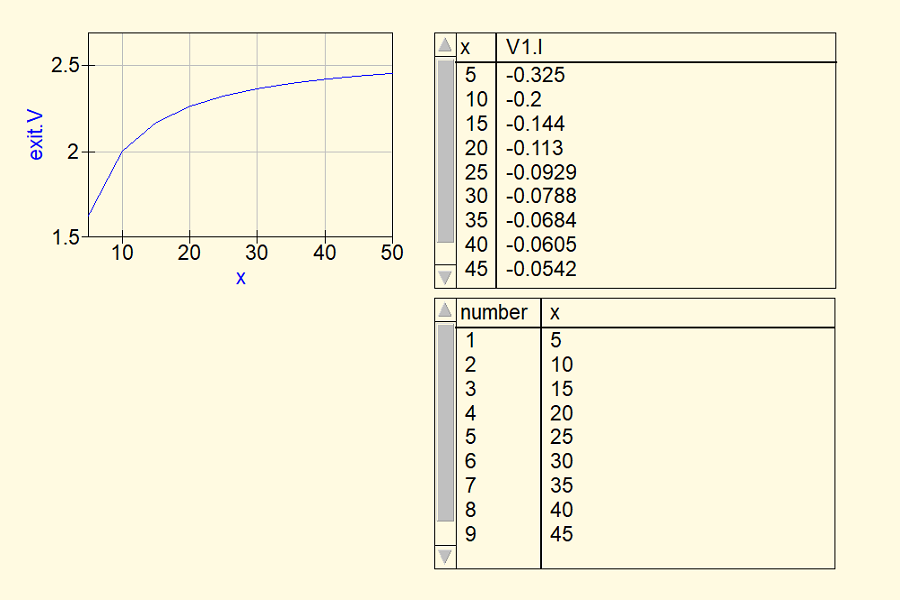
\includegraphics[width=.9\linewidth]{qucs_2}
\caption{Plot with Cartesian coordinates, tabular view of currents flowing from points V1.1 and x.}
\label{i:qucs}
\end{figure}

%Bibliographic references
\begin{thebibliography}{9}
\bibitem{geda} 
Ales Hvezda. 
\textit{gEDA}
\\\texttt{http://www.geda-project.org/}

\bibitem{qucs} 
Michael Margraf, Stefan Jahn.  
\textit{Quite Universal Circuit Simulator}
\\\texttt{http://qucs.sourceforge.net/}

\end{thebibliography}

\end{document}
